\subsubsection{Scopo}
Include le attività e i compiti svolti per creare il prodotto.
\subsubsection{Aspettative}
Le aspettative della corretta implementazione del processo sono:
\begin{itemize}
		\item realizzare un prodotto finale conforme alle richieste del proponente e che soddisfi le attività di validazione e verifica;
		\item fissare gli obiettivi di sviluppo;
		\item fissare i vincoli tecnologici.
\end{itemize}

\subsubsection{Descrizione}
In accordo con lo standard \iso{ISO/IEC 12207}, il processo di sviluppo è composto dalle attività di:
\begin{itemize}
		\item analisi dei requisiti;
		\item progettazione;
		\item codifica.
\end{itemize}

\subsubsection{Analisi dei requisiti}
 \paragraph{Scopo dell'attività}
  Individuare i requisiti del progetto dalle specifiche del capitolato e tramite incontri con il pro-
  ponente. Tale attività produrrà un documento redatto dagli analisti, i quali avranno cura di elencare i casi d'uso e i requisiti. Tale documento permette di
 capire le scelte di progettazione effettuate.
 \paragraph{Aspettative dell'attività}
 L'attività fissa come scopo la creazione di un documento che elencherà e rappresenterà i requisiti richiesti dal proponente.
 \paragraph{Descrizione dell'attività}
 Tutti i requisiti analizzati, utilizzando le specifiche del capitolato e consultando i proponenti negli
incontri effettuati, vanno specificati nell'\ARdocRR. Per analizzare e trovare i
requisiti (si utilizza la tecnica dei casi d'uso). Il tracciamento dei requisiti avviene tramite ... 
 \paragraph{Studio di fattibilità}
 Il \RESP{} di progetto deve organizzare delle riunioni preventive, per permettere lo scambio
di opinioni tra i membri del gruppo sui capitolati proposti. Il documento prodotto da queste
riunioni è lo \SFdocRR , il quale viene realizzato dagli \ANP{}. Essi devono
descrivere i seguenti punti: 
\begin{itemize}
 \item \textbf{Dominio tecnologico e applicativo}: si dà una valutazione prendendo in   considerazione
 la conoscenza attuale delle tecnologie richieste dal capitolato in analisi da parte dei membri  
del gruppo;
 \item \textbf{Interesse strategico}: si valuta l'interesse strategico del gruppo di progetto in relazione
al capitolato in analisi;
 \item \textbf{Individuazione dei rischi}: si analizzano i possibili rischi a cui si può incorrere nel
capitolato in analisi.
\end{itemize}
 \paragraph{Casi d'uso}
 Ogni caso d'uso è così composto:
 \begin{itemize}
  \item codice identificativo;
  \item titolo;
  \item diagramma UML;
  \item attori primari;
  \item attori secondari;
  \item scopo;
  \item descrizione;
  \item precondizione;
  \item postcondizione;
  \item scenario principale;
  \item scenari alternativi.
 \end{itemize}
 \paragraph{Codice identificativo dei casi d'uso}
da decidere
 \paragraph{Requisiti}
 Ogni requisito è così composto:
  \begin{itemize}
  \item codice identificativo;
  \item tipologia;
  \item descrizione;
  \item fonti.
 \end{itemize}
 \paragraph{Codice identificativo dei requisiti}
 da decidere
 \paragraph{UML}
 Viene utilizzata la versione corrente alla stesura del documento , ovvero la 2.5.

\subsubsection{Progettazione}
 \paragraph{Scopo dell'attività}
L'attività di progettazione definisce le linee essenziali della struttura del prodotto software in
funzione dei requisiti individuati dall'analisi. L'obiettivo del processo consiste nella stesura dei
documenti: specifica tecnica e definizione di prodotto.
 \paragraph{Aspettative dell'attività}
Il processo porta alla formazione dei documenti sopra citati, i quali garantiscono affidabilità e
coerenza.
 \paragraph{Descrizione dell'attività}
La progettazione deve rispettare tutti i vincoli e i requisiti concordati tra i componenti del gruppo
e i proponenti. I documenti derivati da questa attività sono:
\begin{itemize}
	\item \textbf{Specifica tecnica}: descrive la progettazione ad alto livello relativa all'architettura dell'applicazione
e dei singoli componenti. Il documento specifica i diagrammi UML ed i design
pattern utilizzati per realizzare l'architettura definendo inoltre i test necessari alla verifica;
	\item \textbf{Definizione di prodotto}: descrive in dettaglio la progettazione di sistema, integrando
quanto scritto nella Specifica Tecnica. Il documento specifica i diagrammi UML e le
definizioni delle classi definendo inoltre i test necessari alla verifica.
\end{itemize}
 \paragraph{Specifica tecnica}
\begin{itemize} 
	\item \textbf{Diagrammi UML}:
	\begin{itemize}
	\item Diagrammi delle classi;
	\item Diagrammi dei package;
	\item Diagrammi di attività;
	\item Diagrammi di sequenza.
	\end{itemize}
	\item \textbf{Design pattern}: devono essere descritti i design pattern utilizzati per realizzare l'architettura. Ogni design
pattern deve essere accompagnato da una descrizione ed un diagramma, che ne esponga il
significato e la struttura;
	\item \textbf{Tracciamento delle componenti}:
	\item \textbf{Test di integrazione}: devono essere definite delle classi di verifica, utili a verificare che ogni componente del
sistema funzioni nella maniera appropriata.
\end{itemize}
 \paragraph{Definizione di prodotto}
\begin{itemize}
	\item \textbf{Diagrammi UML}:
	\begin{itemize}
		\item Diagrammi delle classi;
		\item Diagrammi di attività;
		\item Diagrammi di sequenza.
	\end{itemize}
	\item \textbf{Definizioni delle classi}: ogni classe progettata deve essere descritta in modo da spiegarne lo scopo e definirne le
funzionalità ad essa associate.
	\item \textbf{Tracciamento delle classi}: ogni requisito deve essere tracciato, in modo da poter risalire alle classi ad esso associate. 
	\item \textbf{Test di unità}: devono essere definiti dei test di unità utili a verificare che le componenti del sistema funzionino nel modo previsto.
\end{itemize}

\subsubsection{Codifica}
 \paragraph{Scopo dell'attività}
 Lo scopo dell'attività è l'implementazione del prodotto, concretizzando la soluzione tramite la codifica.  
 \paragraph{Aspettative dell'attività}
 L'aspettativa dell'attività è un prodotto corretto, ovvero stabile, affidabile, funzionale e che soddisfi i requisiti. 
 \paragraph{Descrizione dell'attività}
 L'attività deve rispettare i compiti e gli strumenti espressi nel \PPdocRR.
 \paragraph{Stile}
Le norme di stile saranno specificate in versioni successive di questo documento.
 \paragraph{Versionamento}
 Lo stile di rappresentazione della versione del codice verrà trattato e descritto in versioni successive di questo documento.
 \paragraph{Ricorsione}
 La ricorsione va evitata. Se non risulta accettabile convertirla in iterazione, bisogna fornirne la prova di terminazione e l'analisi del costo in termini di spazio.
\subsubsection{Strumenti}
  \paragraph{Astah}
  Astah è uno strumento di modellazione UML. Verrà quindi usato per la produzione di diagrammi UML. Viene utilizzata la versione 7.0 o superiori.
\begin{figure}[h]
\centering
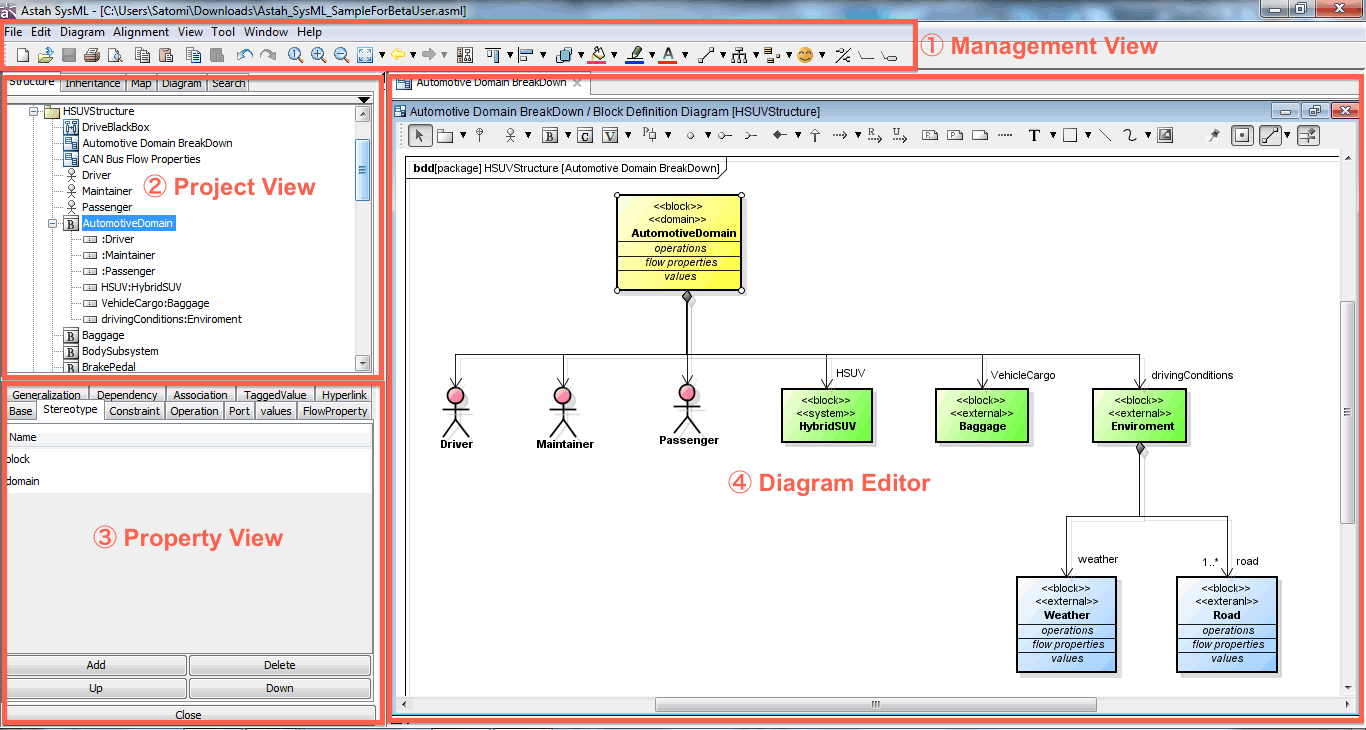
\includegraphics[scale=0.3]{img/astah.png}
\caption{Astah}\label{sec:Figura1}
\end{figure}
 \paragraph{PragmaDB} 
PragmaDB è uno strumento open-source di tracciamento dei requisiti. Verrà quindi utilizzato per semplificare e automatizzare il più possibile l'attività di analisi dei requisiti.



  
